\chapter{Threat Model}
\label{ch:threatmodel}
In this chapter we detail our threat modelling approach, document our iterative process which iterates the threats, identifies mitigations and manages risk.


\section{Adversary}
\label{sec:adversary}
In order to make secure systems, we must always consider the system design and threat given a specified adversary.  For our system, our adversary is a moderate capability Blackhat hacker who seeks to compromise our password system for financial gain.  

\section{Assumptions}
\label{sec:assumptions}
As part of our threat model, we identified several security assumptions which are documented in appendix 1.  Several assumptions demand deeper discussion.
\begin{enumerate}
    \item{\emph{The OS is secure.} While this may seems trivial to note this assumption, a fundamental premise of the password manager design is that the OS functions leveraged by the device such as USB load and clipboard have not been compromised.  If these key OS functions are compromised then any data in transit will be vulnerable to disclosure.  We minimize our attack surface by using volatile memory only and using the USB as our sole source of cryptographic functionality to the maximum extent possible.}
    \item{\emph{The user will physically protect the device.} In our scenario analysis, permanent denial of service will result from loss of the device.  Since we do not provide any backup (in order to minimize the attack surface), it is the user's responsibility to have a disaster plan in case of physical loss.  We are quite confident that passwords will not be compromised in the event of a loss, but a loss also means that a user will no longer have access to the password store.}
    \item{\emph{Our adversary is looking for financial gain.} Additionally, our adversary has the resources to employ moderate BlackHat capabilities but will not engage in any attacks where the attack cost will exceed the expected financial gain.}\sidenote[][]{This means that given our measly financial assets, most attackers will not employ national level attack against our password manager just to confirm how poor we really are!}
These assumptions are pretty straight forward.
\end{enumerate}


\section{Threats}
\label{sec:threats}
In this section we identify the threat to each major element of our
system, usually by using a dataflow diagram.  We conduct a STRIDE analysis on each major data flow or component using the Microsoft Elevation of Privilege game and personal inspection.\sidenote{The elevation of privilege game can be found at \url{https://www.microsoft.com/en-us/SDL/adopt/eop.aspx}}  For each threat we decide whether or not to add it to our risk chart; for similar threats or threats that depend on a similar attack tree we enter only one threat into the risk table but track the remaining threats in the bug table to ensure they are properly managed and mitigated. As we iterated threats, we noted several limitations of the OWASP Risk Management Methodology:
\begin{enumerate}
    \item{The OWASP model places considerable emphasis on non-repudiation.  For our analysis, many of the threats can be realized by simple possession of the USB device which does not require logging of any sort.  Following the risk methodology model without any modification will yield the highest assessment (likelihood) for detectability. In the future we would consider amending the rubric for this particular likelihood factor.}
    \item{The technical impact categories and rubrics were very helpful, however since many of these attacks were aimed at obtaining the USB password, they rated artificially high because the cascade of compromise that resulted in obtaining a password. The rubric for either technical impact or likelihood did not allow for consideration of existing countermeasures or design features in the device.  Again, this resulted in artificially high risk assessments.  For a second iteration, we would recommend including an assessment of design features and countermeasures intended to address the threat or related threat as a better way to better estimate the likelihood of a risk.}
    \item{The business impact categories while useful in a real world exercise were not applicable to this threat model.  In the future we would look at substituting more applicable rubrics in place of the existing business impact factors of the OWASP model.}
\end{enumerate}

In spite of the limitations we discuss, the OWASP model was very useful in drawing our attention to the highest risk threats.  We benefited from using the 5x5 risk matrix as opposed to the 3x3 OWASP risk matrix because we were able to break out threats and risk to a finer degree.

\subsection{Spoofing Threats}
\begin{marginfigure}%
\centering
  
\includegraphics[width=0.33\linewidth]{spoofcard}
  \caption{Spoofing Card from the Elevation of Privilege Game}
  \label{fig:spoofcard}
\end{marginfigure}
Spoofing threats deal with an attacker's ability to masquerade as an individual, process or some other entity in order to gain access to data and systems.  During our first iteration we identified several spoofing threats.

\begin{table}[]
    \centering
    \begin{tabular}{c|c}
         &  \\
         & 
    \end{tabular}
    \caption{Caption}
    \label{tab:my_label}
\end{table}


\subsection{Tampering Threats}
\begin{marginfigure}%
\centering
  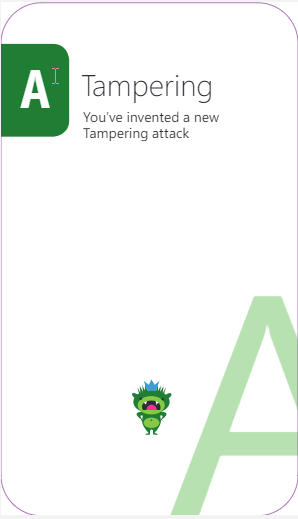
\includegraphics[width=0.4\linewidth]{tampercard}
  \caption{Tamper Card from the Elevation of Privilege Game}
  \label{fig:tampercardcard}
\end{marginfigure}

\subsection{Repudiation Threats}
\begin{marginfigure}%
\centering
  
\includegraphics[width=0.4\linewidth]{repudcard}
  \caption{Repudiation Card from the Elevation of Privilege Game}
  \label{fig:repudcard}
\end{marginfigure}

\subsection{Information Disclosure Threats}
\begin{marginfigure}%
\centering
  
\includegraphics[width=0.4\linewidth]{infodisclcard}
  \caption{Information Disclosure Card from the Elevation of Privilege Game}
  \label{fig:spoofcard}
\end{marginfigure}

\subsection{Denial Of Service Threats}
\begin{marginfigure}%
\centering
  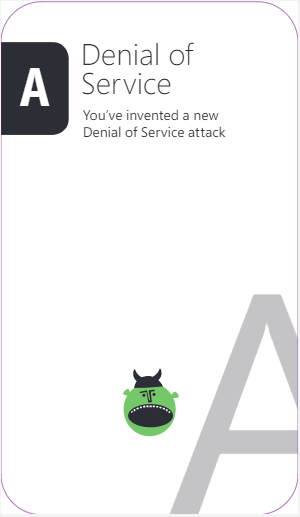
\includegraphics[width=0.4\linewidth]{doscard}
  \caption{Denial of Service Card from the Elevation of Privilege Game}
  \label{fig:doscard}
\end{marginfigure}

\subsection{Elevation of Privilege Threats}
\begin{marginfigure}%
\centering
  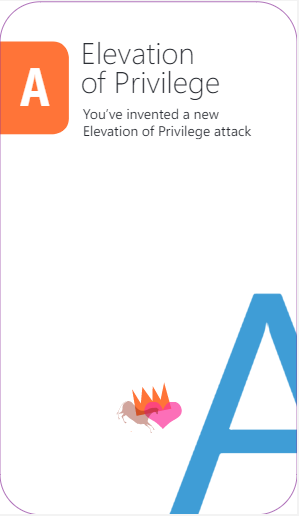
\includegraphics[width=0.4\linewidth]{eopcard}
  \caption{Elevation of Privilege Card from the Elevation of Privilege Game}
  \label{fig:eopcard}
\end{marginfigure}


\section{Threat Summary by Highest Risk}

\subsection{Risk Table}

\subsection{Risk Matrix}

\section{Attack Trees}
We conduct an analysis of each threat using a threat tree.

\section{Highest Risks and Their Mitigaitons}




